\begin{figure}[t]
\centering
\begin{tikzpicture}[scale=4.2]
\begin{scope}
\draw[->] (-0.05,0) -- (0.9,0) node[right] {$t$};
\draw[->] (0,-0.03) -- (0,0.78) node[above] {$t^2$};
\draw[thick,gray,domain=-0.02:0.86,smooth,variable=\t] plot ({\t},{\t*\t});
\coordinate (a1) at (0.25,0.0625); \coordinate (a2) at (0.75,0.5625);
\coordinate (c1) at (0,0); \coordinate (c2) at (0.625,0.390625);
\draw[very thick,blue] (a1) -- (a2);
\draw[very thick,red,dashed] (c1) -- (c2);
\fill[blue] (a1) circle (0.012) node[below right] {$\tfrac14$};
\fill[blue] (a2) circle (0.012) node[right] {$\tfrac34$};
\fill[red] (c1) circle (0.012) node[below left] {$0$};
\fill[red] (c2) circle (0.012) node[above left] {$\tfrac58$};
\fill (0.5,0.3125) circle (0.014);
\node[anchor=north west] at (0.52,0.30) {\small $(\tfrac12,\tfrac5{16})$};
\node at (0.42,0.72) {\small (a) interleaving};
\end{scope}
\begin{scope}[xshift=1.15cm]
\draw[->] (-0.05,0) -- (0.9,0) node[right] {$t$};
\draw[->] (0,-0.03) -- (0,0.78) node[above] {$t^2$};
\draw[thick,gray,domain=-0.02:0.86,smooth,variable=\t] plot ({\t},{\t*\t});
\coordinate (a1) at (0,0); \coordinate (a2) at (0.75,0.5625);
\coordinate (c1) at (0.25,0.0625); \coordinate (c2) at (0.5,0.25);
\draw[very thick,blue] (a1) -- (a2);
\draw[very thick,red,dashed] (c1) -- (c2);
\fill[blue] (a1) circle (0.012) node[below left] {$0$};
\fill[blue] (a2) circle (0.012) node[right] {$\tfrac34$};
\fill[red] (c1) circle (0.012) node[below right] {$\tfrac14$};
\fill[red] (c2) circle (0.012) node[below right] {$\tfrac12$};
\node at (0.42,0.72) {\small (b) nested};
\end{scope}
\end{tikzpicture}
\caption{Moment pairs $(\E y,\E y^2)$ of distributions on a two-point set
form the chord of the parabola between the two points. Solid: $A$;
dashed: $C$. (a) The sets $A=\{\tfrac14,\tfrac34\}$ and $C=\{0,\tfrac58\}$ of
Proposition~\ref{prop:path-gap} interleave,
the chords cross at $(\tfrac12,\tfrac5{16})$, and the glued pair relaxation
has value $0$. (b) Nested sets $A=\{0,\tfrac34\}$ and $C=\{\tfrac14,\tfrac12\}$:
the chords do not meet, and by
Theorem~\ref{thm:interleave} the glued relaxation attains the true minimum
$\delta^2/2$ in the direction of $\Phi$.}
\label{fig:chords}
\end{figure}
